\subsection{External Hybrid-Method Results}
\label{subsec:external_method_results}
All 1620 additional model fits complete without fitting warnings, giving 3240 decision-rule evaluations. Provenance checks verify exact synthetic-count matching and original-retention matching in all 270 geometry--corruption--replication combinations. The original and copied generators agree exactly in 270 data-role checks. No-intervention and ordinary SMOTE results are reused from the earlier targeted extension.

Table~\ref{tab:external_control_means} reports equally weighted means of the nine setting-specific differences. SMOTE-ENN's default-rule advantage over no intervention is $0.2436$ for LR and $0.0555$ for SVM; after validation-based threshold selection, the corresponding differences are $-0.0026$ and $-0.0030$. Against ordinary SMOTE, selected-threshold mean differences are $-0.0003$ and $-0.0026$. Thus, the operating-point explanation is relevant to an external hybrid method as well, but does not explain every pairwise outcome.

\begin{table*}[t]
\caption{External Control: Descriptive Mean SMOTE-ENN-minus-Comparator G-mean Differences}
\label{tab:external_control_means}
\centering\small
\begin{tabular}{llrrc}
\hline
Model & Comparator & Default & Selected & Selected interval directions\\
\hline
LR & No intervention & +0.24357 & -0.00262 & 0/2/7 \\
LR & SMOTE & -0.01097 & -0.00030 & 1/0/8 \\
LR & Count-matched SMOTE & +0.04104 & -0.00031 & 0/3/6 \\
LR & Count + retention matched & +0.01031 & +0.00040 & 1/0/8 \\
SVM & No intervention & +0.05548 & -0.00301 & 3/5/1 \\
SVM & SMOTE & -0.00473 & -0.00257 & 0/5/4 \\
SVM & Count-matched SMOTE & -0.00198 & -0.00476 & 0/5/4 \\
SVM & Count + retention matched & +0.01146 & +0.00582 & 3/2/4 \\
\hline
\end{tabular}
\par\smallskip\footnotesize Each mean weights nine settings equally. Direction counts are above zero / below zero / including zero for individual 95\% paired intervals, not adjusted significance decisions. Count matching uses post-editing synthetic counts; retention matching additionally uses the exact surviving original observations. Intervals are setting-specific; no pooled interval over the nine dependent settings is claimed.
\end{table*}

Count matching alone gives selected-threshold mean differences of $-0.0003$ for LR and $-0.0048$ for SVM. Matching original retention as well changes these to $+0.0004$ and $+0.0058$. For SVM with dispersed corruption, SMOTE-ENN exceeds the retention-matched control in Gaussian, moons, and circles settings, with respective mean differences of $0.01018$, $0.01601$, and $0.03062$; their individual paired intervals lie above zero. Boundary-near corruption instead produces adverse SVM differences for Gaussian and circles. These outcomes do not establish uniform superiority.

Editing also changes intervention quality. Averaged across geometries under dispersed corruption, corrupted-endpoint use declines from $0.5741$ before editing to $0.3656$ among retained synthetics. However, approximately $14.2\%$ of correctly labeled minority originals are removed, and original-removal precision is approximately $14.2\%$. Under boundary-near corruption, endpoint contamination changes little ($0.5944$ to $0.5864$). These summaries distinguish label-related intervention errors from classification outcomes and do not establish synthetic-label correctness.

% Optional figure: copy external_control_intervals.png into the manuscript figures folder.
\begin{figure*}[t]
\def\xfigwd{\columnwidth}
\centering
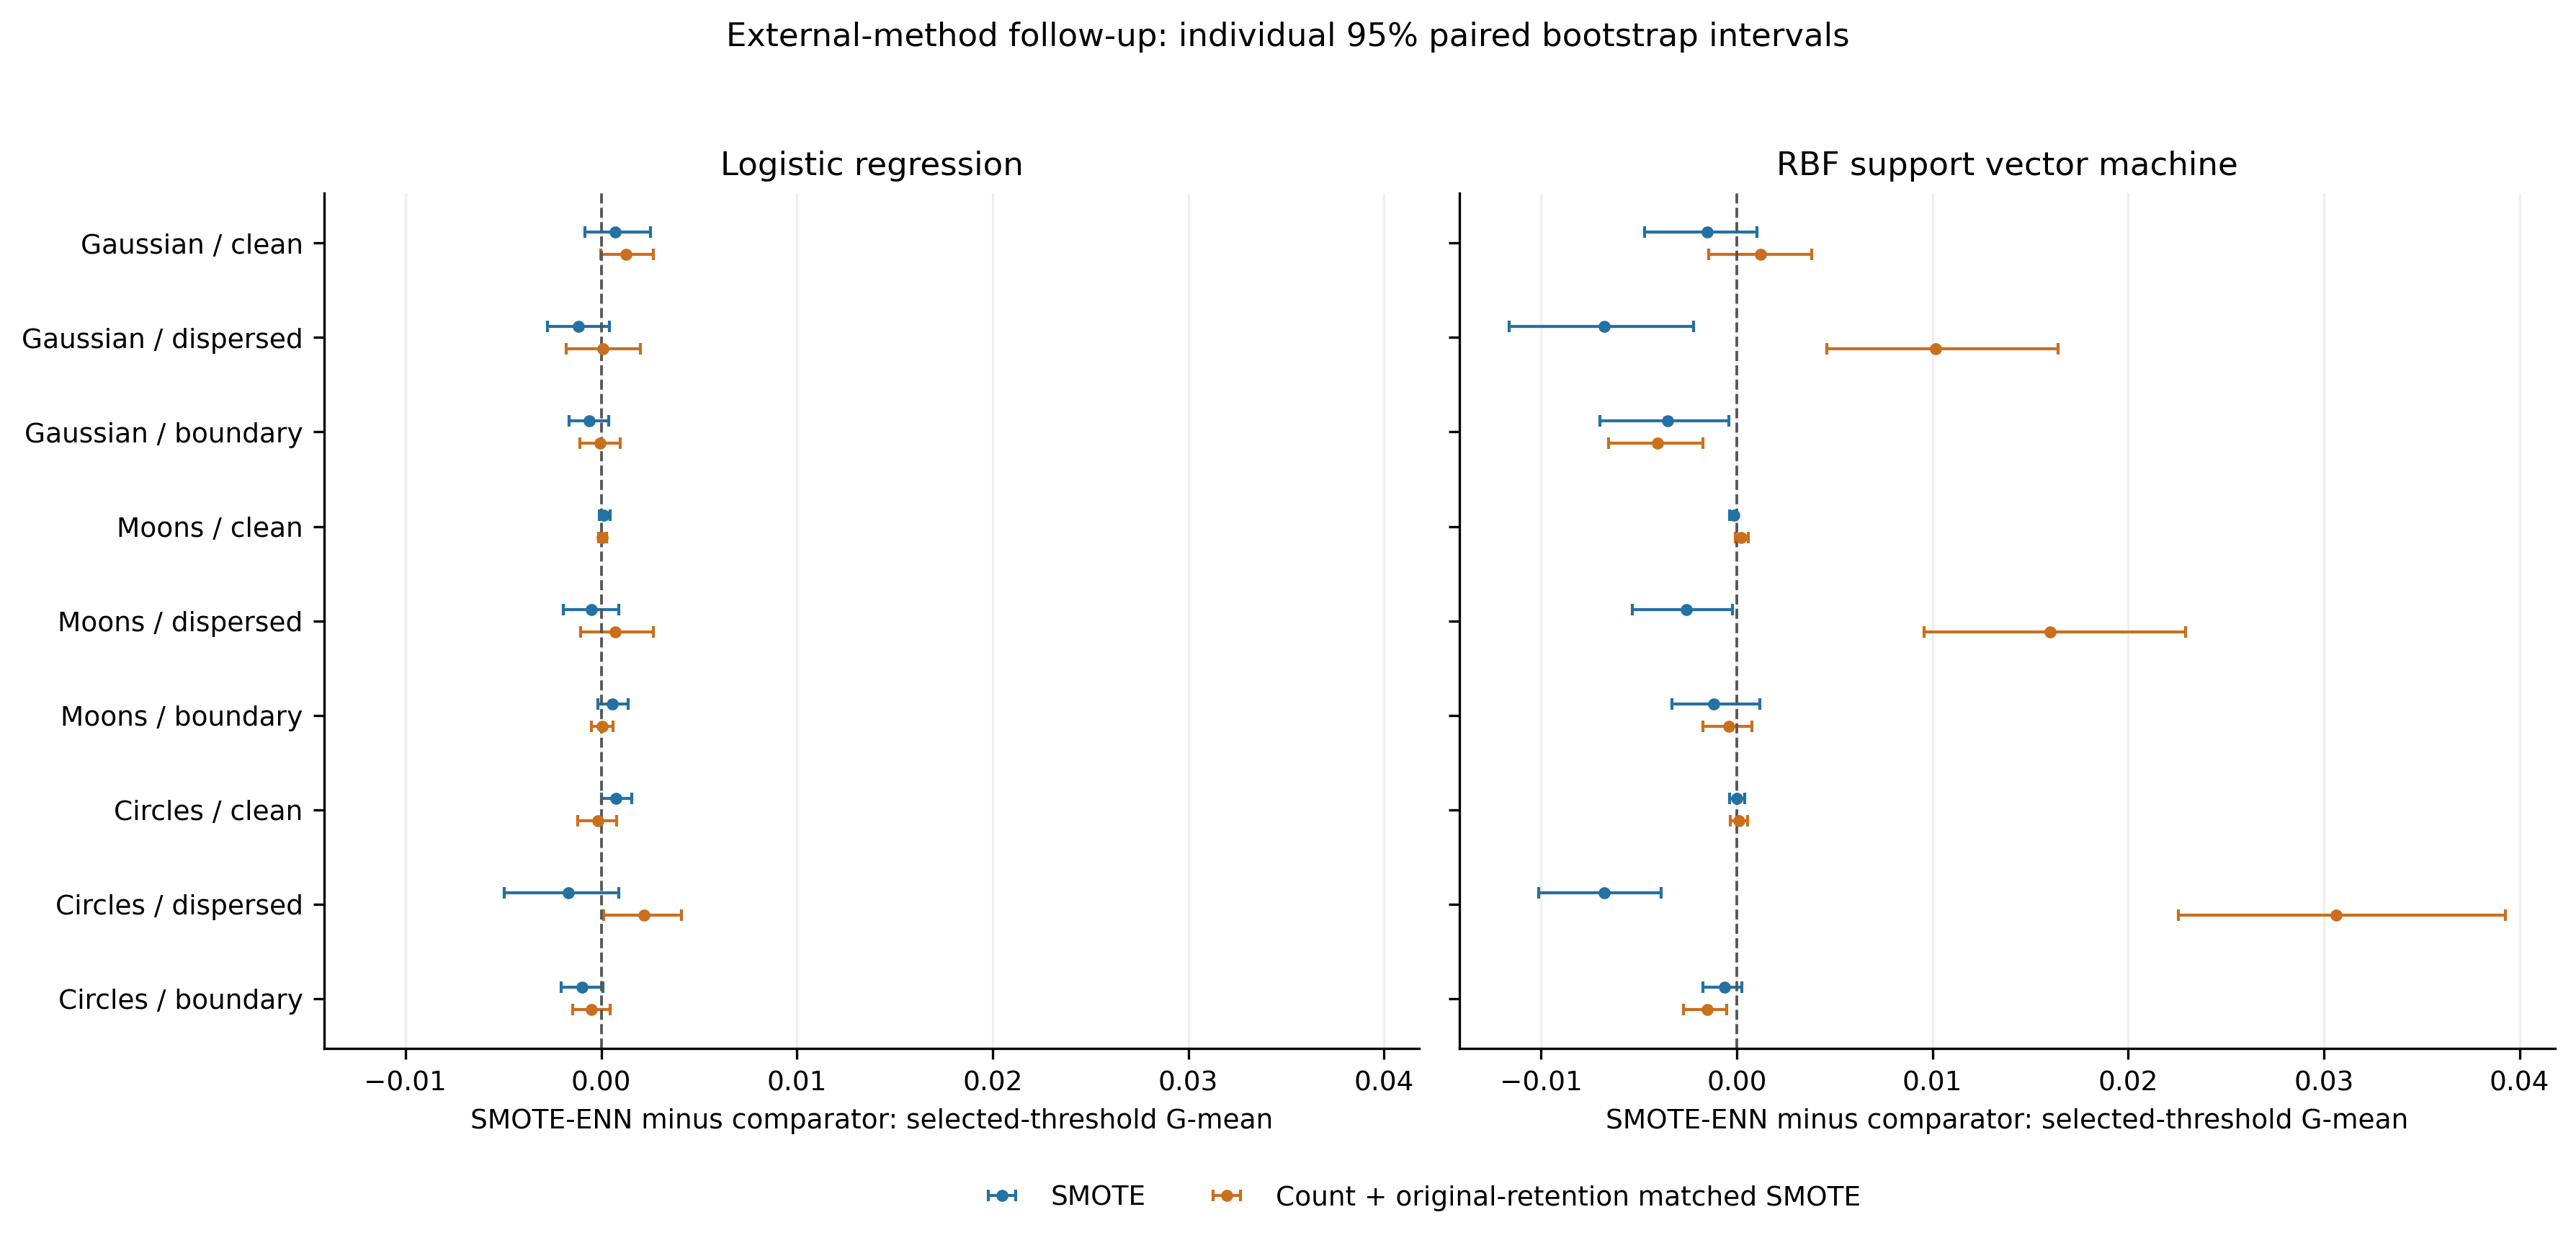
\includegraphics[width=\textwidth]{external_control_intervals.png}
\caption{External hybrid-method follow-up. SMOTE-ENN-minus-comparator G-mean after validation-based threshold selection; bars are individual exploratory 95\% paired bootstrap intervals based on 30 replications and 5000 resamples. Matching original retention is additional to matching synthetic count. These intervals do not provide simultaneous coverage.}
\label{fig:external_control_intervals}
\end{figure*}
